\section{Designing a compiler for fluxional compliancy} \label{section:compiler}

% The section \ref{section:model} of this paper describes the fluxional execution model, a framework to run web application in a distributed environment.
% This section explains the compiler we developed to transform a subset of classic web application to be compliant with the execution model previously described.
% This transformation unveils two problems due to the differences between a web application and the execution model.
% In the first section, a distributed system is defined by the parallel execution of its parts, and the distribution of its memory.
Current Web applications are mostly written in Java. The langage proposes both data encapsulation and threading model, that ease the development of distributed applications.
Yet, Java framework for developing efficient applications are complex systems that impose new API\cite{Coward2003} to the developers.
Since 2009, \textit{Node.js}\cite{Dahl} provides a simple Javascript Web programming system.
We focus on this promising environment for its initial simplicity and efficiency.
We develop a compiler that transforms a simple javascript application into a fluxional system compliant to the architecture described in section \ref{section:model}.
As javascript forbids user-space thread API, a javascript application is developed as a mono-threaded application.
Moreover, in Javascript  the memory is hierarchical and the root scope may be accessed by any function, which leads to bad component isolation.
Our compiler finds fluxions into most of Web-based Javascript application.
It finds component isolation through the analyzer step and memory consistency through the linker step.
We do not target all Javascript Web-based application but if we are able to transform either some part of applications or 50\% of currently running applications without external developer help, we expect a real execution gain in a cloud environment.
The rest of this section describes the two parts of the compiler.
% A classic web application is not composed of many independent parts, and relies on a central memory.
% We wants to parallelize the execution of a mono-thread application into many independent parts, and to distribute the central memory among these parts.
% We describe a compiler as a solution to this problem, hence capable to transform a classic web application into a distributed system.
% In this section, we describe the two compilation steps responsible of resolving parallelization and distribution.
Section \ref{section:analyzer} explains how the \textit{analyzer} detects rupture points in the web application to mark out the independent parts.
Section \ref{section:linker} explains how the \textit{linker} resolves the missing dependencies due to the distribution of the central memory.

% TODO move this
% The compiler reuses some tools from the Javascript community.
% The compiler and these tools follow the specification for an intermediate representation of the Javascript source code from the Mozilla Javascript Parser API\cite{JsAST}.
% \textit{Esprima}\cite{esprima} parses the source and generate an Abstract Syntax Tree (AST).
% The compiler analyze and modify this tree by traversing it using \textit{Estraverse}\cite{estraverse}.
% \textit{Escope}\cite{escope} extracts function scopes and variables declaration from the tree.
% At the end of the compilation chain, the compiler uses \textit{Escodegen}\cite{escodegen} to transform AST back into Javascript source code.

\subsection{Analyzer : execution parallelism} \label{section:analyzer}

The parallelization of programs is a trending problem to leverage the multiple cores available on highly parallel architectures.
The Sun programming guide\footnote{\raggedright http://docs.oracle.com/cd/E19455-01/806-5257/6je9h032b/index.html} defines \textbf{parallelism} as \textit{a condition that arises when at least two threads are executing simultaneously}, and \textbf{concurrency} as \textit{a condition that exists when at least two threads are making progress. A more generalized form of parallelism that can include time-slicing as a form of virtual parallelism}.
\textbf{Asynchronism} is a condition that arises when a communication point continues processing an independent thread of execution while waiting for the answer to his request.

Promises\cite{Liskov1988}, as well as \textit{Node.js} callbacks, are abstractions that transform blocking synchronous operations into non-blocking asynchronous operations.
This asynchronous operation run concurrently with the main thread, until the requested value is computed, and the main thread can continue the computation needing this value.
This asynchronism splits the execution in two concurrent execution paths, one that needs the requested value and one that doesn't.
We call rupture points, points where the execution flow forks in two concurrent paths due to asynchronism.
These points mark out the limits between the independent parts of an application.
 
The analyzer detects rupture points to break the application into independent parts.
In this section, we define what a rupture point is, and how we detect them.

\subsubsection{Rupture points}

Rupture points represent a fork in the execution flow due to an asynchronous operation.
They are composed of an asynchronous function, and a callback to handle the result of the operation.
The two execution flows are the following instructions after the asynchronous function, and the instructions in the callback.
Listing \ref{lst:hello} is an example of rupture point in a simple application.
A rupture point is an interface between two application parts.

\begin{code}[Javascript, caption={Example of a rupture point : an asynchronous function call, \texttt{fs.readFile()}, with a callback parameter, \texttt{function display}},label={lst:hello}]
var fs = require('fs');
fs.readFile(__filename, function display(err, data) {
  console.log('>> second concurrent execution path');
  console.log(err || data.toString());
})
console.log('>> first concurrent execution path');
\end{code}

% \begin{code}[Javascript, caption={Example of a rupture point : an asynchronous function call, \texttt{app.get()}, with a callback parameter, \texttt{function reply}},label={lst:hello}]
% var app = require('express')();
% app.get('/', function reply(req, res) {
%   res.send('Hello World :)');
% });
% app.listen(8080);
% console.log('server listening to 8080');
% \end{code}

There are two types of rupture points - basic and special - illustrated respectively in figure \ref{fig:basicrp} and \ref{fig:specialrp}.
In these figures, the two concurrent execution paths distributed in two application parts are indicated by \circled{1} and \circled{2}.

\textbf{Basic rupture points} represent a simple continuity in the execution flow after a finite asynchronous operation, such as reading a file in listing \ref{lst:hello}.
The function calls from basic rupture points mark the interface between the current application part and the next one.
This frontier is placed before the call to the asynchronous function, but after the resolution of the arguments.
The result of this asynchronous operation probably being a voluminous object, this placement allow the asynchronous function call to occur in the same application parts as the callback, avoiding the transfer of this voluminous result, as illustrated in figure \ref{fig:basicrp}.

\begin{figure}[h!]
\begin{center}
  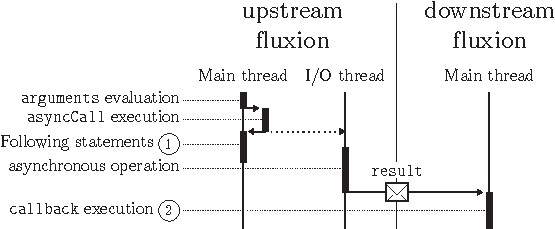
\includegraphics[width=\linewidth]{ressources/basicrp.pdf}
  \caption{Basic rupture point interface. \textnormal{The interface is placed before the asynchronous operation, to avoid moving the result from one application part to another.}}
  \label{fig:basicrp}
\end{center}
\end{figure}

\textbf{Special rupture points} differ in that they are on the interface between the whole application and the outside, continuously handling incoming user requests, like \texttt{app.get()} in listing \ref{lst:rupturepoints}.
The callbacks of these functions indicate the input of a data stream in the program, and the beginning of a chain of application parts following this stream.
The \textit{start} rupture points will later be used to monitor the load from incoming external requests.
Because the asynchronous function is called only once, while the callback is triggered multiple times, this interface is placed between the two, as illustrated in figure \ref{fig:specialrp}.

\begin{figure}[h!]
\begin{center}
  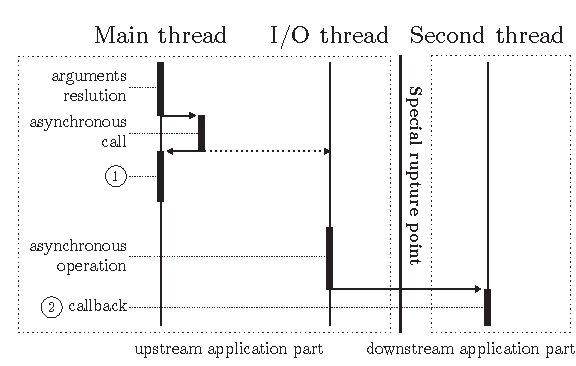
\includegraphics[width=\linewidth]{ressources/specialrp.pdf}
  \caption{Special rupture point interface. \textnormal{The interface is placed after the asynchronous operation, for the downstream application part to be triggered at each event.}}
  \label{fig:specialrp}
\end{center}
\end{figure}

In the following, basic rupture points are called \textit{post}, and special rupture points are called \textit{start}


\begin{code}[Javascript, caption={Example of an application presenting the two types of rupture points : a \texttt{start} with the call to \texttt{app.get()}, and a \texttt{post} with the call to \texttt{fs.readFile()}},label={lst:rupturepoints}]
var app = require('express')();
var fs = require('fs');

app.get('/:filename', function handleRequest(req, res) {
  fs.readFile(__dirname + '/' + req.params.filename, function reply(err, data) {
    res.send(err || data);
  })
});

app.listen(8080);
console.log('server listening to 8080');
\end{code}

\subsubsection{Detection}

Detecting a rupture point requires detecting its two components : the asynchronous function and the callback function.

\textbf{Asynchronous functions}\\
The compiler is prebuilt with module names exposing asynchronous function, like the \textit{express}, and the \textit{fs} module in listing \ref{lst:rupturepoints}.
To detect asynchronous calls, the compiler register variables holding such modules, building a dictionary of the asynchronous function call name.
In listing \ref{lst:rupturepoints}, the compiler register both variables \texttt{app} and \texttt{fs}.
When the compiler encounter a call expression, it compare its callee name to the dictionary to spot asynchronous functions.

\textbf{Callback function}\\
For each asynchronous call expression detected, the compiler test if an argument is a function.
Some callback functions are declared \textit{in situ}, and are trivially detected.
For every other variable identifier, we track the declaration up to the initialization value to detect functions.

\textbf{Variable tracking}\\
To detect both the asynchronous function and the callback function, the compiler needs to statically track the states of the variables.
Missing rupture points by false negatives in the detection is sub-optimal, but false positives eventually produce an unstable compilation result.
Therefore, the detection needs to be as accurate as possible to screen out false positives.
We use a technique similar to a Program Dependency Graph (PDG)\cite{Ferrante1987} to track changes in the value of variables.


\subsection{Linker : memory distribution} \label{section:linker}

Because of the central memory, parallelism is not sufficient for an application to be distributed.
The compiler needs to distribute the memory into the application parts for the application to be compliant with the fluxional execution model.
In Javascript, scopes are nested one in the other up to the all-enclosing global scope.
Each function creates a new scope containing variables local to itself, and is chained to the scope of the parent function.
The child function can access variables in the scope of the parent functions, up to the global scope.
Rupture points are found in between scopes, linking application parts in message streams.
A rupture point placed between a child scope and its parent break a chain of scope, and makes the child unable to access its parent as expected, eventually leading the application to crash during execution.
The linker analyzes how scopes are distributed among the application parts to detect and resolve conflicts between these scopes.
Depending on how the shared variable is used in the functions scopes, there are different situations to resolve.
In the following, we explain the different cases of inconsistency emerging from the partitioning of a central memory.

\subsubsection{Signature}

The signature is the part of a message containing all the variables to send downstream.
If a variable is needed for read-only access by at least one downstream application part, it is added to the signature of the rupture point.
As fluxions are chained one after another, a fluxion must provide every dependency for the next one, even if some of this dependencies are not needed by the current application part.
These dependencies must be passed fluxion after fluxion from the producing fluxion to the consuming fluxion.
The code inside the application part is modified for the signature's references to point to the message signature instead of the function scope.

\subsubsection{Scope}

The scope is the name given to the persisted memory of a fluxion.
It holds the variables declared outside, but needed for modification in only one application part.
If one of these variables needs to be read by another application part downstream, this variable becomes part of the signature sent downstream.
An example of such a variable is a request counter. Initialized to 0 in the global scope, the counter is incremented for each request.
This counter would be in the scope of the application part handling requests reception, and sent downstream for visit metrics processing.

\subsubsection{Sync}

If a variable is needed for modification by more than one distributed application parts, this variable needs to be synchronized between the fluxions' scopes.
Memory synchronization in a distributed system is a well-known problem.
According to Brewer's theorem, formalized by Seth Gilbert and Nancy Lynch \cite{Gilbert2002}, it is impossible for a distributed computer system to simultaneously provide all three of the following guarantees : Consistency, Availability, Partition tolerance.
Partition tolerance can't be avoided in a distributed system\cite{codahale2010}, so the only possible tradeoff is between consistency and availability.
These two tradeoffs are defined in the literature as ACID (Atomicity, Consistency, Isolation, Durability) for consistency over availability, and BASE (Basically Available, Soft state, Eventual consistency)\cite{Fox1997} for availability over consistency.
The objective for this compiler is to be able to transform a subset of web application with a satisfying result.
We choose to keep both consistency and availability, therefore we must sacrifice partition tolerance and keep these application parts together.

\subsection{Guidelines and Future work}

This compiler aims at transforming efficiently a subset of Javascript web applications presenting a specific syntax and design.
In this section, we describe briefly the main situations to avoid for an efficient compilation.
The compilation silently fails if a variable holding a callback or a module is assigned a second time.
The variable tracker is unable to track accurately all the modification of a variable to detect this situation and screen out the corresponding rupture point.
The compiler is still unable to track the value of dynamically resolved variables.
If this variable is then used as a callback, the compiler won't be able to detect it as a rupture point.
Variables poorly encapsulated or used too globally tighten dependencies accross the code.
In these conditions, the compiler is unable to efficiently break the application in parts, resulting in poor distribution and scalability.
The \textit{express} module provides only a factory to create the object holding the asynchronous functions.
The compiler is still unable to understand this scheme, and fails if the factory isn't called directly from the \texttt{require}, like in \ref{lst:rupturepoints}.
Most of the limitations described above are caused by the variable tracker described in section \ref{section:analyzer}, being in an early stage of development.
We are currently in the process of extending further the reach of this component to extend the subset of compilable applications.

We believe that our work will keep scalability concerns out of the way from the development team, who could then focus on the core logic of their application.
In future developments of this project, we aim at making application dynamically reactive to the load of user requests.
By monitoring only the input stream, the \texttt{start} rupture points, we believe it is possible to infer the load propagation through the application.
Using analogy with fluid dynamics, each fluxion is like a pipe, traversed by a fluid of user requests.
The input and output throughput of this pipe could be calibrated before production use, generating an approximative model of the application reaction to input load.
Using this model, we want to make the application's reorganize itself in a cluster to handle pikes in the user request throughput.

\subsection{Compilation example}

% For copyright reason, the compiler source code is kept private along with the tests we used.
To illustrate the compiler features, we compiled a very simple, yet representative, application.
It sends back its own source, presenting both a special and a basic rupture point.
It sends a download counter as well to illustrate the use of fluxion's own memory.
Source and results are available on github\cite{flx-example}.
The file \texttt{result.flx} is the result of the compilation in our high-level fluxional language.
The file \texttt{result.js} is the result of the compilation targeting the fluxional execution model.
